\documentclass[11pt,a4paper]{article}
\usepackage[hyperref]{acl2020}
\usepackage{times}
\usepackage{amsmath}
\usepackage{graphicx}
\usepackage{amsfonts}
\usepackage{float}
\usepackage{enumitem}
\usepackage{latexsym}
\usepackage[english]{babel}
\usepackage{natbib}

\usepackage[activate={true,nocompatibility},final,tracking=true,kerning=true,spacing=true,factor=1100,stretch=10,shrink=10]{microtype}

\graphicspath{{./images}}
\bibliographystyle{unsrtnat}

\title{A Survey on Conversational AI in\\
Task-oriented and Question-Answering tasks}

\author{Sanchit Nevgi \\
  College of Information and Computer Sciences \\
  University of Massachusetts, Amherst \\}

\begin{document}
\maketitle

\begin{abstract}
  Ubiquitous deep learning approaches have led to the advent of neural Conversation AI systems, also known as dialogue systems. Modern dialogue system can be distinctly categorized into 3 modules --- A Natural Language Understanding (NLU), Dialogue Manager (DM), and Natural Language Generation (NLG). In this survey, we investigate the evolution of diaogue systems, from hand-crafted rules and statistical approaches to recent end-to-end data-driven neural methods. Specifically we focus on task-oriented dialog systems, where the dialog agent works toward a specific goal, for example, booking movie tickets as well as open-domain question answering.
\end{abstract}

\section{Introduction}

Advancements in deep learning have led to improved performance in dialogue systems. \textit{A dialogue agent} is an entity that you can interface with via voice/text that has certain capabilities. These capabilities can be broadly classified into three categories \cite{Gao2019NeuralAT} as,

\begin{enumerate}[leftmargin=*, label={}]
  \item \textbf{Question \& Answering}: QA agents allow users to query large-scale Knowlege Bases (KB-QA) or document collection in natural lanaguage (text-QA). In the real-world, text-QA agents are most commonly used in search engines such as Google, Bing, while KB-QA are widely used in voice assistants.
  \item \textbf{Task completion}: Task-oriented systems work towads a well-specified goal, such as movie ticket booking, usually in a multi-turn fashion. The dialogue system keeps track of the dialogue state, uses information supplied by user to constrain search, prompts user for required information for task completion.
  \item \textbf{Social dialogue}: The agent needs to converse seamlessly with users, provide useful recommendations. A good dialgoue agent should demonstrate emotional connect with the user. For example, showing excitement when user shares good news, empathy when user is feeling sad, etc.
\end{enumerate}

In this review, we study the evolution of the approaches used in building an effective dialogue agent, with an emphasis on task-oriented goals. Traditional approaches for building task-oriented dialogs relied on hand-crafting features \cite{Core1997CodingDW, Jelinek1976SpeechRB} and casting dialgoue as an optimal decision making problem \cite{Young2013POMDPBasedSS, Kaelbling1998PlanningAA}. These approaches are unable to adapt to new domains, aren't robust to \textit{user paraphrasing}, and semantic word similarity. Further, in these approaches, the system is comprised of several modules (NLU, NLG, etc) that are optimized independently shown in Figure \ref{fig:pipeline}. Recent approaches utilize neural network models that are trained end-to-end.

\section{Dialogue as an Optimal Decision making task}

We briefly review of Reinforcement Learning (RL) and Markov Decision Processes. A comprehensive overview in RL is out of scope for this review. Interested readers are referred to the excellent work by \cite{Sutton1988ReinforcementLA, Kaelbling1996ReinforcementLA}

\medskip \noindent \textbf{Reinforcement Learning}: Reinforcement Learning (RL) is a learning paradigm where given an agent in an environment, the agent has to learn to take optimal decisions. Every action is followed by an immediate reward, which is a signal to the agent of its performance. Each iteration of the agent in the environment is described by,
\begin{enumerate}[leftmargin=*]
  \item The agent observes the environment's current state $s_t$ and takes an action $a_t$
  \item The environment transitions to the next state $s_{t+1}$, distributed according to transition probability $P(\cdot | s_t, a_t)$
  \item The agent recieves an immediate reward $r_t$ post transition.
\end{enumerate}
The agent-environment interaction is often modeled as a discrete-time Markov decision process, described next.

\begin{figure}[H]
  \centering
  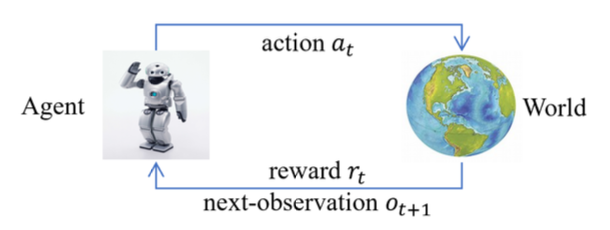
\includegraphics[width=0.4\textwidth]{images/rl.png}
  \caption{Reward system in RL environment}
  \label{fig:rl}
\end{figure}

\noindent \textbf{Markov Decision Processes (MDP)}: A Markov Decision Process is used to describe an environment for reinforcement learning, where the environment is fully observable. An MDP is a Markov Reward Process with decisions, it’s an environment in which all states are Markov \cite{Sutton1999BetweenMA}. 

\medskip \noindent \textbf{Partially Observable MDP (POMDP)}: A Spoken Dialog System (SDS) can be cast as a Partially Observable MDP \cite{Williams2007PartiallyOM, Young2013POMDPBasedSS}. A POMDP can be developed to encompass a complete dialog system and serves as a basis for optimization. It can integrate uncertainty in the form of statistical distributions.

Formally, a POMDP is defined as a tuple ($\mathcal{S}, \mathcal{A}, \mathcal{T}, \mathcal{R}, \mathcal{O}, \gamma, b_0$) where 

\begin{itemize}[leftmargin=*]
  \setlength\itemsep{0em}
  \item $\mathcal{S}$ is a set of all states
  \item $\mathcal{A}$ is a set of actions
  \item $\mathcal{T}$ defines a transition probability $P(s_t|s_{t-1}, a_{t-1})$
  \item $\mathcal{R}$ defines the expected immediate real-valued reward, \item $\mathcal{O}$ is a set of observatoins
  \item $\mathcal{Z}$ defines an observation probability $P(o_t|s_t, a_{t-1})$
  \item $\gamma$ is the geometric discount factor $0 \leq \gamma \leq 1$
  \item $b_0$ is the initial belief state.
\end{itemize}

\begin{figure}[h]
  \centering
  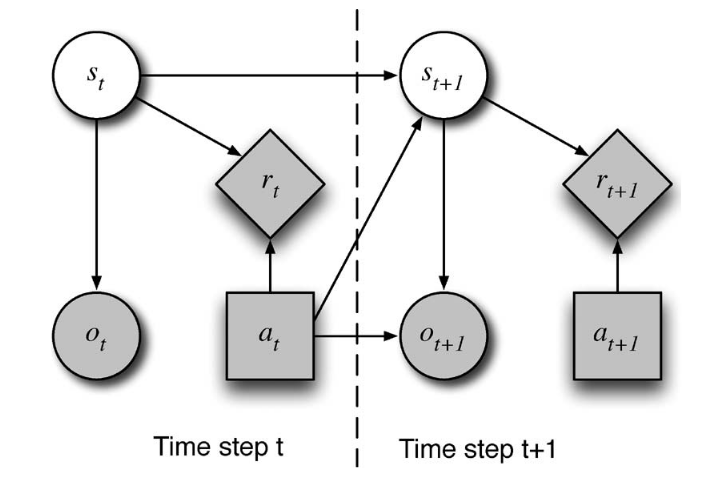
\includegraphics[width=0.5\textwidth]{images/pomdp.png}
  \caption{A Partially Observed Markov Deicison Process}
\end{figure}

\begin{figure*}[t]
  \centering
  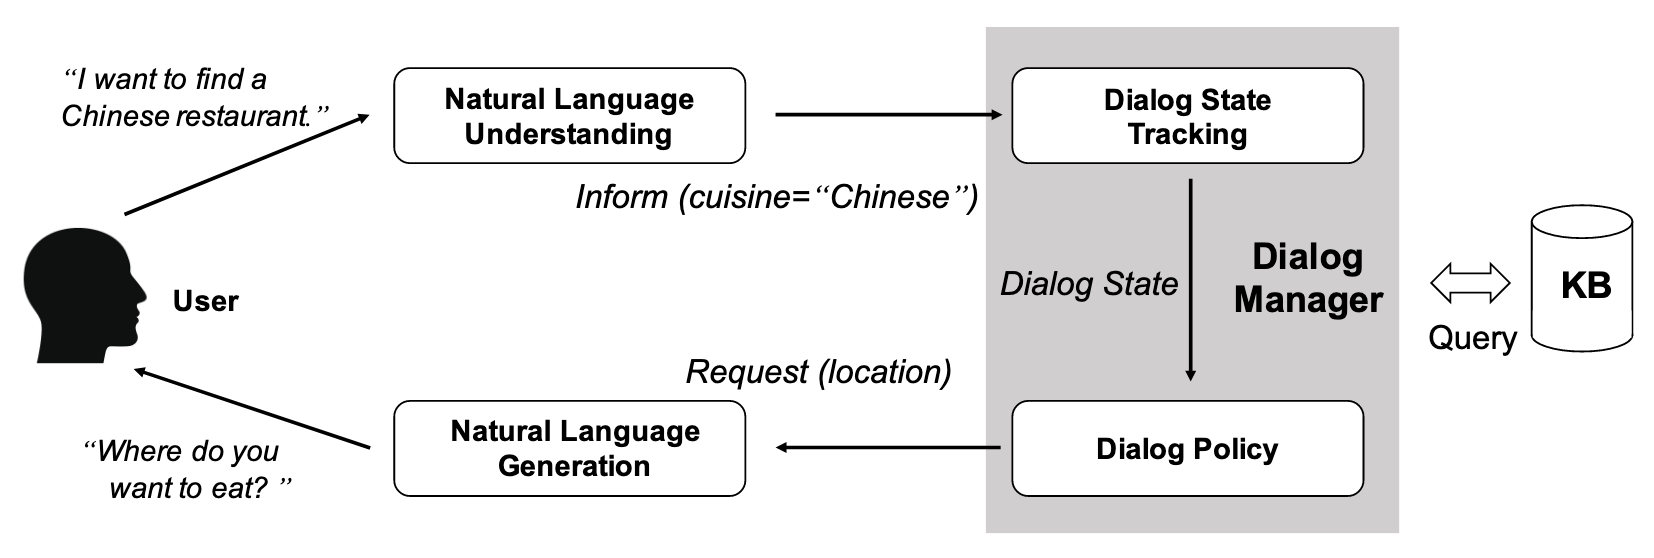
\includegraphics[width=\textwidth]{images/pipeline_framework.png}
  \caption{Modules in an NLP system}
  \label{fig:pipeline}
\end{figure*}

At each time step $t$, the world is in some unobserved state $s_t$. A distribution over possible states called belief states $b_t$ is maintained where $b_t(s_t)$ is the probability of state $s_t$. Based on this, the model selects an action $a_t$, receives an observation $o_{t+1}$.
Given an existing belief state $b_t$, the last system action $a_t$, and the new observation $o_{t+1}$, the new update belief state $b_{t+1}$ is given by 

\begin{equation}
  \begin{split}
    b_{t+1}(s_{t+1}) &= \eta P(o_{t+1}|s_{t+1}, a_t) \\ & \cdot \sum\limits_{s_t} P(s_{t+1}|s_t, a_t) b_t(s_t)
  \end{split}
\end{equation}

where $\eta$ is the normalization constant. The system action is determined by policy $\pi$. It is commonly represented by a deterministic mapping from belief states to actions $\pi(b) \in \mathcal{A}$ or stochastically via a distribution over actions $\pi(a|b) \in [0,1]$\

The discounted sum of rewards expected by starting in belief state $b_t$, using policy $\pi$ is given by the \textit{value function} as 

\begin{equation}
  V^{\pi}(b_t) = \mathbb{E} [r_t + \gamma r_{t+1} + \gamma^2 r_{t+2} + ...]
\end{equation}

A similar quantity is the Q-function $Q^\pi (b,a)$, which gives the expected discounted sum of rewards if action a is taken given belief state b, followed by policy $\pi$. The \textit{optimal policy} $\pi^*$ is one that maximizes $V^\pi$ to yield $V^*$, also known as the \textit{Bellman optimality} equation. Including an explicit Bayesian model of uncertainty and by optimizing the policy via a reward-driven process, POMDPs provide a framework for modeling dialog managers \cite{Young2010TheHI}. These models are optimized by maximizing the expected cumulative sum of rewards at each turn.

For real-world applications, the computation over all possible states becomes intractable and applying a direct solution is very difficult. Various approximation techniques have been propsed. 

The principal components of a conversational Spoken Dialog System are shown in Figure. At each turn $t$ , an SLU component converts each spoken input into an abstract semantic representation called \textit{user dialog act} $u_t$. The \textit{system} updates its internal state $s_t$ and determines the next system act via a decision rule $a_t = \pi(s_t)$, known as \textit{policy}. The system act is converted to speech using NLG component.

The posterior probability of the belief state after each user input is updated via Bayesian inference in a process known as \textit{belief monitoring}. The design of the belief state allows user behaviour to be captured as model priors and the inference process is able to exploit the full distribution of recognition hypothesis. By maintaining a belief distribution over all states, the system is effectively pursuing all possible dialog paths in parallel, choosing the next action based on all the most likely state but all all states. The explicit representation of state and policy action allow dialog design to be incorporated by associating rewards with state-action pairs.

\smallskip \noindent \textbf{Belief State Representation and Monitoring}:
In a practical application, the state must encode the user's utterance $u_t$, the history context $h_t$ and the user's goal $g_t$. Therefore, the state is a combination of three components $s_t = f(g_t, u_t, h_t)$. Reasonable independence assumptions are made regarding the conditional independencies of the model.

\smallskip \noindent \textbf{Challenges}: The \textit{state-action} space is extremely large, which makes real-time Bayesian inference rather challenging. The exact policy learning for POMDPs is intractable and approximation techqniques have to be used. Further, learning requires real-world users which are expensive to aquire and time-consuming. Hence, building capable user simulators are required for learning.

\section{Natural Languge Generation}

Natural Language Generation is vital to convert a communication goal, selected by the Dialogue Manager, into natural language. Traditionally rule/template-based methods were used for generation, with the transition to data-driven approaches. We briefly review recent approaches to NLG.

\subsection{\textsc{Seq2Seq} models}

Also known as encoder-decoder architecture, these models are fundamental to language modeling tasks, such as machine translation and dialogue response generation. They are typically implemented using recurrent architectures such as RNNs and their counterpart, LSTMs \cite{Hochreiter1997LongSM}. In these models, semantic representations of the input text tokens are passed through the \textit{encoder}, through a series of transforms, yeilding a hidden representation of the input. The output is generated token-by-token using this representation, which is known as the \textit{decoder}. 

\begin{figure*}[t]
  \centering
  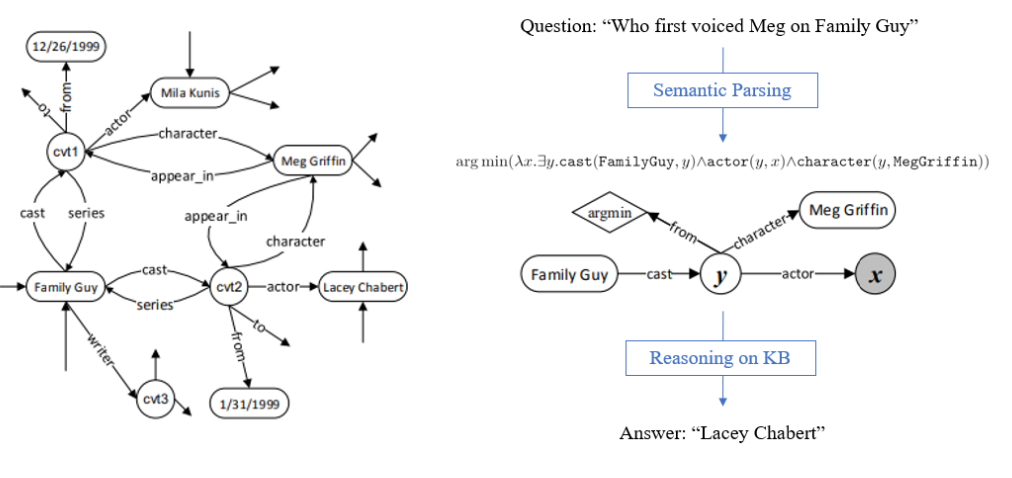
\includegraphics[width=\textwidth]{images/kg.png}
  \caption{(Left) Semantic Parsing for KB-QA on a subgraph of Freebase. (Right) A question in its logical form using $\lambda$-calculus}
\end{figure*}

\subsection{Contextualized word embeddings and Transformers}

Recurrent models faced the issue of keeping track of long-term context, which prompted the use of attention. \cite{Vaswani2017AttentionIA} showed that only using the attention mechanism was sufficient for model generation performance, called as the Transformer architecture. Subsequently, the BERT model \cite{Devlin2019BERTPO} used bi-directional tranformers to get pre-trained contextualized word embeddings that possessed deep language understanding.

\section{Question Answering}

Traditionally Conversational Question Answering relied on creating and maintaining hand-engineered rules. With the rise of deep learning, methods have been develoed to automate this process. There are two main types of QA agents - KB-QA agents query a large-scale Knowledge Base (KB) to retrieve information. text-QA agents use Information Retrieval techniques on a document collection, to obtain a ranked list of relevant documents. Google Search, Bing are examples of text-QA agents.

\subsection{Knowledge Bases}

A Knowledge Base is a structured store of facts, usually in graph format. Typically, a KB consits of \textit{subject-predicate-object} triples $(s,r,t)$, where $s, t \in \mathcal{E}$ are entities and $r \in \mathcal{R}$ is the relation between the entities. Some popular KBs are Freebase \cite{Bollacker2008FreebaseAC}, which has since been integrated into Google Search, ConcpetNet \cite{Speer2016ConceptNet5A} which is huge graph consiting of approximately 8m concepts and relations between them.

\noindent State-of-the-art symobilic approaches to reasoning over KB are based on \textit{semantic-parsing} \cite{Berant2013SemanticPO, Einolghozati2019ImprovingSP}, where a question is mapped to its formal meaning representation and then translated to a KB query. Applying symbolic KB-QA to a very large KB is challenging due to --- Paraphrasing in Natural Language and the search complexity.

\section{Task-Oriented Systems}

With recent advancements in on-device machine learning, voice assistants such as Google Assitant, Siri, Alexa have promulgated. These systems assist users in completing tasks such as making restaurant reservations, booking movie tickets, setting an alarm. These tasks differ from the QA in that they work toward a specific goal over multiple turns. We review the various components in Task-oriented systems with emphasis on recent neural approaches.

\medskip \noindent \textbf{Slot-filling dialogues}: The user and the system converse with the goal of \textit{slot-filling}. The system must collect all the necessary information from the user to formulate an appropriate query. In the movie ticket booking domain, some examples of slots are \texttt{movie-name, time, price, location}. Slots are \textit{informable} if the user can provide the \textit{slot-value}, used to constrain the search; or slots are \textit{requestable}, where the user can ask the value of the slot from the system (eg \texttt{phone\_number}).

\medskip \noindent \textbf{Dialogue Act}: The interaction between the user and the system, known as the dialogue act, can be modeled as a agent-environment problem in Reinforcement Learning, where the user is equivalent to the environment and the system is the agent. Briefly, at each turn, the agent keeps track of the dialogue state, then takes an action based on the current state. The user responds with an utterance and an immediate reward is computed to measure the quality of the turn. We elaborate these steps in more detail further.

The architecture of task-oriented dialog systems can be broadly divided into two categories --- Pipeline and End-to-end approaches. The pipeline system consists of 4 components,

\begin{enumerate}
  \setlength\itemsep{0em}
  \item Natural Language Understanding
  \item Dialogue State Tracking
  \item Dialogue Policy
  \item Natural Language Generation
\end{enumerate}

NLU maps to structured semantic representation. A popular schema for semantic representation is \textit{dialog act}, which consists of intent and slot-values.
The NLU task is mapped into intent-detection and slot extraction. Intent detection is framed as classification problem and slot-extraction is framed as sequence labeling task.

\begin{figure}[h]
  \centering
  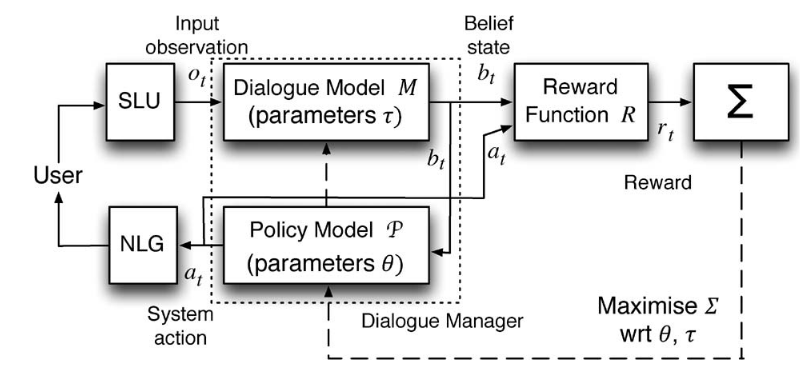
\includegraphics[width=0.4\textwidth]{./images/pomdb_dialog_manager.png}
  \caption{POMDP-based dialog manager}
\end{figure}

\subsection{Learning End-to-End Task-oriented Dialog}

Learning task-oriented dialogs end-to-end requires defining a user simulator and a dialogue agent. Next, we define baseline tasks to measure neural methods's performances. Traditional dialog systems in task-oriented dialogs require lot of domain-specific handcrafting, which makes it difficult to scale. These limitations are mitigated in end-to-end trained systems. \cite{Bordes2016LearningEG} shows that, compared to hand-crafted slot-filling baseline, end-to-end dialog system based on \textit{Memory networks} \cite{Sukhbaatar2015EndToEndMN} can reach promising, but imperfect performance and can even perform non-trivial operations.

Successful goal-oriented dialog systems model coversation as partially observable Markov deicsion processes. Require hand-crafted features for state and action space representations, restricting to narrow domains. To measure the performance of task-oriented dialog systems, 5 common tasks have been proposed. They are,

\begin{itemize}[leftmargin=*,label={}]
  \setlength\itemsep{0em}
  \item Task 1 - Issuing API calls
  \item Task 2 - Updating API calls
  \item Task 3 - Displaying options
  \item Task 4 - Providing extra information
  \item Task 5 - Full dialogs
\end{itemize}

In \cite{Bordes2016LearningEG}, the authors use a restaurant KB, which has \texttt{name, cuisine, location, price range, address, phone number}. Each example in the dataset comprises of dialog utterances from user and bot, as well as API calls and the resulting facts. They split the KB into two, disjoint sets of \textit{cuisines}, and \textit{locations}, to test the models capability to handle Out-of-Vocabulary scenario. The dialog systems are evaluated in a ranking, not a generation setting. At each turn of dialog, they test whether they can predict bot utterances by selecting candidates.

Further, the model is evaluated on real concierge service where the dialogs are shorter, and the vocabulary more diverse. Some of the findings are that the set of user requests is much wider compared to dataset, from managing restaurant reservation to asking for recommendations. Also, the users do not stay focused on the request. The facts about restaurants are not structured like KB and finally the users and operators make typos, spelling and grammatical erros.

Models:

Rule-based systems - Used hand-crafted rules such as word matches, positions in dialog, entity detections, dialog state.

Classic IR models - 
  TF-IDF match - For each possible candidate response, compute the matching score between input and response. Score is TF-IDF weighted cosine similarity between the bag-of-words of input and response.
  Nearest neighbour - Find most similar conversation in the training set and use that response. Word overlap as scoring method. Sorted by decreasing co-occurence frequency.

Supervised embedding models - Predict next response given the previous conversation. Scored for input $x$ as $f(x, y) = (Ax)^TBy$. Trained with margin ranking loss

Memory Networks -

Word embeddings fail with entities. Embeddings use approx word match. Cannot handle OOV words.
Solution - match type features. Augment vocab with 7 words (cuisine, location, etc)

\subsection{Building End-To-End dialogue systems using Generative Hierarchical Neural Network Models}

\cite{Serban2015BuildingED} investigate the task of open-domain, conversational dialogue systems. They make Use heirarchical recurrent encoder-decoder neural network. POMDPs are popular, and demonstratively work well for limited examples. Further, non-task-oriented sytems can be used to develop user simulators, which can be further used to generate dialogue datasets to train POMDP models. The dialogue response generation can be modeled as a translation task.Although it is more difficult due to numerous plausible responses and lack of phrase alignment between user utterance and response.

Dialog is viewed as sequence of utterances where each utterance comprises of tokens. The architecture consitsts of an \textsc{Encoder-RNN}, which maps each utterance to an utterance vector. It is the hidden state obtained after last token is processed. A Context-RNN iteratively processes each utterance vector. The hidden state of the \textsc{Context-RNN} represents state of the dialogue system. It is passed to the \textsc{Decoder-RNN} to predict the next utterance. The \textbf{HRED} is hypothesized to be superior to RNN because (1) the Context-RNN allows model to represent common ground between speakers and (2) Number of computational steps between utterances is reduced. \cite{Serban2015BuildingED} show that Hierarchical Recurrent model outperforms n-gram based model and the baseline neural networks. They infer that using a large external monologue corpus to initialize word embeddings, and a large non-dialogue corpus for pre-training improves model performance. Finally they conclude that MAP outputs produce generic, but conversationally acceptable responses while stochastic samples from model produced diverse dialogues.

\begin{figure*}[t]
  \centering
  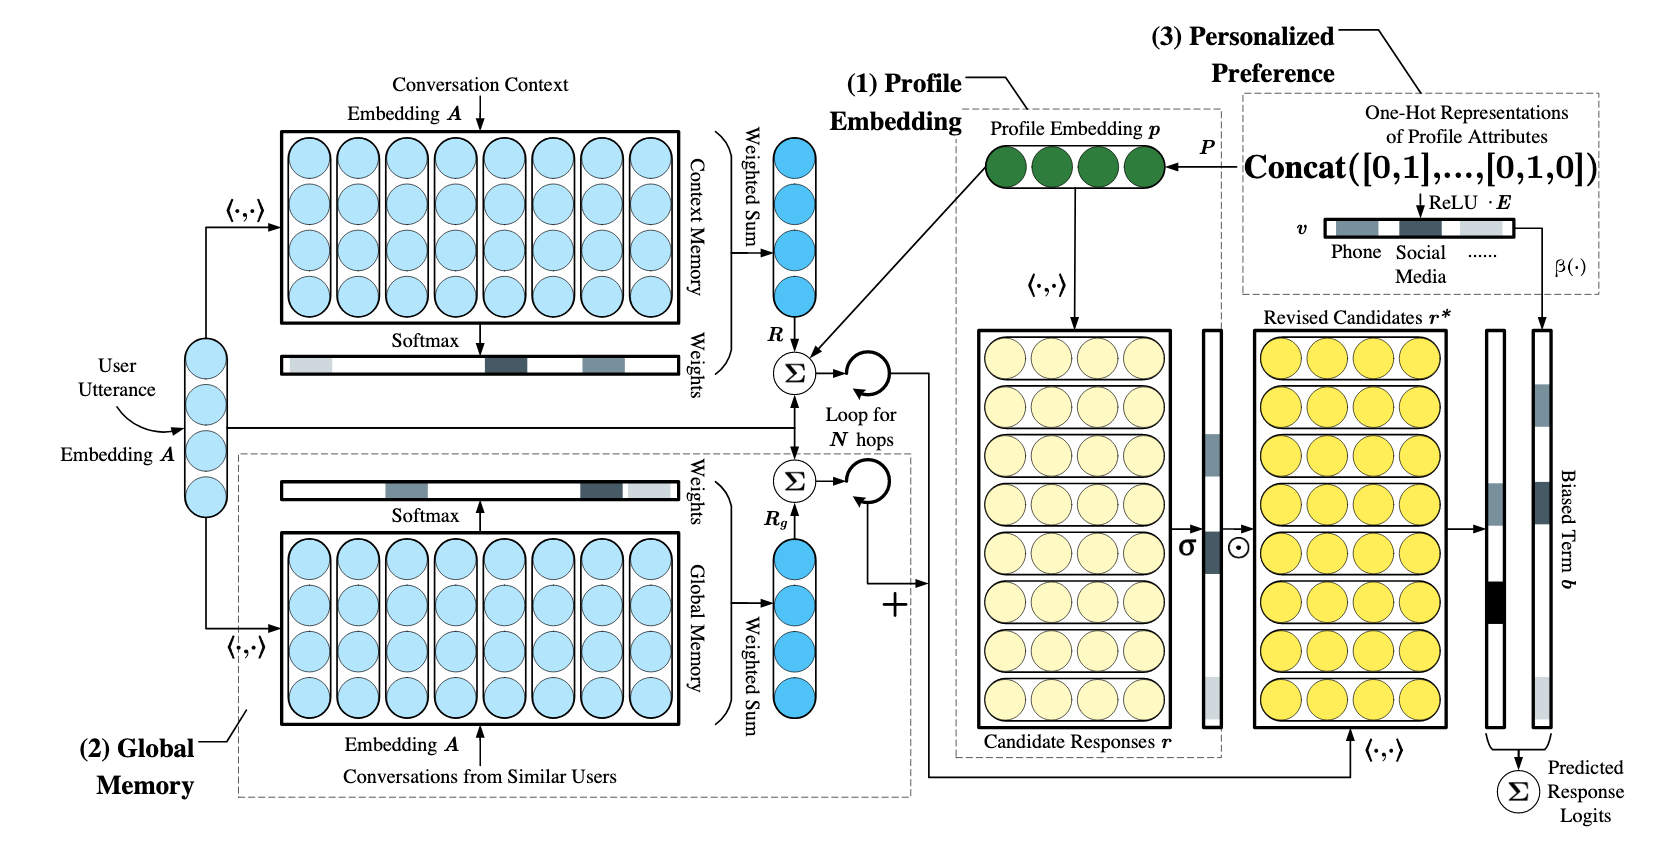
\includegraphics[width=\textwidth]{images/personalized.png}
  \caption{\textsc{Personalzed MemN2N} architecture}
\end{figure*}

\subsection{Neural Belief Tracker: Data-Driven Dialogue State Tracking}

\cite{Mrksic2016NeuralBT} proposes an end-to-end trained DST module known at the \textit{Neural Belief Tracker}. A \textit{belief tracker}, estimates the user's goal at every step of the dialog. They mitigate two issues with traditional approaches to building DST, namely that NLU models require large amount of training data and hand-crafting lexicons for capturing liguistic variation in users's language is cumbersome.

Using recent advances in \textit{representation learning}, Neural Belief Tracking (NBT) framework reasons over pre-trained word vectors, learning to compose them into distributed representations of user utterances and dialogue context. The \textit{dialogue state tracking} component serves to interpret user input and update the \textit{belief state}, which is the system's internal representation of teh state of the conversation. The dialogue system is supported by \textit{domain ontology}, which describes the range of user intents the system can process. The ontology defines a collection of slots and the values each slot can take.

The task is non-trivial due to lexical variation, dynamics of context and noisy Automated Speech Recognition (ASR) output. Traditional approaches use separate modules to handle lexical variability in single dialogue turn. However the turn-level SLU and cross-turn DST can be coalesced into a single model, but they rely on manually constructed semantic dictionaries.

Some systems use template-based matching systems while others train independent binary models that decide if slot-value pair was expressed in user utterance. SLU has been treated as sequence labeling problem.

The proposed Neural Belief Tracking model uses pre-trained vectors. The input consists of the system dialogue acts preceding the user input, the user utterance, a single slot-value pair it needs to make a decision about. To perform belief tracking, NBT model iterates over all candidate slot-value pairs and decides which ones have just been expressed by the user. \textit{"I'm looking for good pizza"} entails \textsc{Food=Italian}.

\smallskip \noindent \textbf{Representation Learning module}:
The vector embeddings for unigram, bigram and trigram are concatenated and projected to a fixed-size representation. The canditate slot-value pair and user utterance interact through the \textit{semantic decoding} module. The slot and value representation are concatenated, projected to the same size at user utterance vector and finally a similarity score is computed.

To conclude, the NBT couples Spoken Language Understanding and Dialogue State Tracking without relying on hand-crafted semantic lexicons. Further, the model performance improves with the semantic quality of underlying word vectors.

\section{Learning Personalized End-to-End Goal-Oriented Dialog}


Existing works on dialog systems only take into account the conversation content, neglecting the user personality. \cite{Luo2019LearningPE} proposes using a \textsc{ProfileModel}, which encodes user profiles into distributed embeddings and a \textsc{PreferenceModel} captures user preferences over KB. 

Modern approaches train dialogue systems end-to-end \cite{Vinyals2015ANC, Sukhbaatar2015EndToEndMN}. They are directly trained on past dialogs, without domain assumptions. Some common limitaions are the model's (1) inability to adjust language style according to the user (2) lack of dynamic conversation policy based on interlocutor's profile (3) inability to handle ambiguities in user requests. Psychology studies have shown that during a dialog, humans adapt dialog style according to the interlocutor, which enhances conversational efficiency. An exisiting challenge is how to integrate user profile to generate personalized messages.

The \textsc{Profile Model} learns user personalities with distributed profile representations and uses a global memory to store conversation context from users with similar profiles. The \textsc{Preference Model} learns user preferences among ambiguous candidates by building a connection between user profile and knowledge base. These models are integrated into \textsc{MemN2N} network. A common approach to leveraging personality in recent works is using a conditional language model as the response decoder. Existing literature \cite{Li2016APN} focuses on personality in social bots with limited work in task-oriented personality dialogues.

\medskip \noindent \textbf{Notation}: A user profile is represented by $n$ attributes $\{(k_i, v_i)\}^n_{i=1}$, where $k_i$ and $v_i$ denote the key and value of the $i$-th attribute. For example \texttt{\{ (Gender, Male), (Age, Young) \}}. The values are represented as one-hot vectors. A complete \textit{user profile} $\hat{a}$ is obtained by the concatenation of all such one-hot representations.

\medskip \noindent \textbf{ProfileModel}: A profile embedding of the \textit{user profile} is obtained by linear transformation $p = P\hat{a}$. The query $q$ in a \textsc{MemN2N} model plays a key role in reading the memory and choosing the response. At each turn, the profile embedding is incorporated into the query update as

\begin{equation}
  q_{i+1} = q_{i} + o_i + p
\end{equation}

\noindent where $o_i$ is the ouput at the $i$-th hop.

\medskip \noindent \textbf{Global Memory}: Users with similar profile should expect a similar response for a particular request. The personalized information of similar users is incorporated into global memory module. The global memory is similar in structure to the \textsc{MemN2N} model, with the difference that the contents of memeory are history utterances from similar users instead of current coversation.

\section{Evaluation}

Existing measures of evaluation either prevent repoducibility, as different human annotators (Mechanical Turks) would have difference experiences or that the metrics don't correlate with human judgements. Automatic evaluation of the dialogue systems is still an activie area of research. 

Individual components of the system, such as the Natural Langauge Understanding module, may be evaluated using traditional techniques such as accuracy, precision/recall, BLEU scores. However, to get a holistic view of the performance of the entire system, they are insufficient. A common metric used is the \textit{task success rate}, which tracks whether the dialog agent correctly fulfilled the task (booked movie tickets, reserved a table, etc). \cite{Williams2007PartiallyOM}.

Human evaluation is the most accurate measure of the system performance. However, it is expensive to operate on a large scale. Recently, \cite{Adiwardana2020TowardsAH} proposed a new human-evaluation metric known as Sensibility and Specificity Average (SSA). The authors used a 2.6B parameter \textsc{Seq2Seq} model with Evolved Transformer, trained on 40B words. The SSA metric was shown to highly correlate to \textit{perplexity}, which is easier to compute.

\section{Challenges in Neural Task-oriented dialog}

Neural approaches for task completion is advancing at a rapid pace \cite{zhang2020recent}. The frontier in model performance is pushed every day by bigger and better models. However, it is important to consider the data efficiency of these modesl to facilitate dialog system modeling in low-resource settings. A major feature of task-oriented dialog is its emphasis on multi-turn state-action dynamics. Faster and exact policy learning for modeling multi-turn dynamics is essential. Similary, building models that adapt to new domains with reasonable accuracy are cruicial. Lastly, integrating domain ontology knowledge into the dialog model remains a challenge.

\nocite{*}
\bibliography{acl2020}

\end{document}
